\title{\vspace{160px} \textbf{\huge{Telecommunication Theory}} \\\vspace{17.5px} \LARGE{Lab report 5}  \vspace{10px}}
\author{Alessandro Trigolo}
\date{December 11, 2023}

\begin{document}
\maketitle \newpage

\section*{Objective}
The laboratory’s goal is to implement and analyze the effectiveness of the matched filter receiver implemented in the three modulation techniques (BASK, BFSK and BPSK), already explained during laboratory work 3. This kind of receiver uses the \textbf{convolution integral} to properly detect the received symbol. The idea behind
this operation is rather simple: the convolution integral takes a known input sample signal, like the signal of the 1-symbol, and shifts it along all the received - and disturbed - signals. By aligning the shifted sample with parts of the disturbed signal, the convolution integral significantly enhances the likelihood of identifying the corresponding symbol during the detection.


\lstset{style = MATLAB}
\section*{Source code and plots}
The source code provided in this section has to be appended to the code produced during laboratory 3 so there won't be any explanations regarding the above-mentioned code. Alongside the lines of code, there will be some explanatory comments to make the lab 5 source code more readable.

\subsection*{Task 1}
The first thing to do is to implement the matched filter receiver source code for the three modulation techniques. Two methods can be used to compute the convolution integral. The first one is to use the MATLAB function \texttt{conv} and then truncate the signal to get the convolution integral. The second method is to use the MATLAB \texttt{filter} function which won't need the final truncating. In both cases, the code is much shorter than the optimal correlator receiver thanks to these built-in functions.

For the BASK and the BPSK techniques the 1st approach was followed: the few things to do are to flip the carrier signal $s_0$ and then compute (and truncate) the newly convoluted signal.

\begin{lstlisting}
% flip the carrier to make the convolution
s0_flipped = fliplr(s0);

% Perform convolution
convolution_signal = conv(s0_flipped, BPSK_with_noise);

% truncating the convoluted signal
convolution_signal = convolution_signal(1:length(BPSK_with_noise));
\end{lstlisting}

\noindent For the BFSK technique the code has to compute the convolution for the two carrier signals, $s_1$ and $s_2$, which are associated with the 1 and the 0 symbols. In this case, the 2nd method was implemented so there was no need to truncate the signal.

\begin{lstlisting}
% flip the carriers to make the convolution
s1_flipped = fliplr(s1);
s2_flipped = fliplr(s2);

% output of the matched filter
convolution_signal_1 = filter(s1_flipped, 1, BFSK_with_noise);
convolution_signal_2 = filter(s2_flipped, 1, BFSK_with_noise);
\end{lstlisting}


\subsection*{Task 2}
The second task asked to plot on one image the disturbed signal and the optimal correlation receiver signal: the \texttt{subplot} function was utilized. The script is very similar to the three modulation techniques, so it is shown only the script used for the BFSK modulation, which is the more complex one.

\begin{lstlisting}
% plot the disturbed signal
subplot(311), plot(BFSK_intervals, BFSK_with_noise), grid on; 
xlabel('Time, sec'), ylabel('BASK signal with noise'); % labels
ylim([-4, 4]); % limits

% plot 1st matched filter signal
subplot(312), plot(BFSK_intervals, convolution_signal_1), grid on; 
xlabel('Time [s]'), ylabel('1st matched filter'); % labels
ylim([-ylimit, ylimit]); % limits

% plot 2nd matched filter signal
subplot(313), plot(BFSK_intervals, convolution_signal_2), grid on; 
xlabel('Time [s]'), ylabel('2nd matched filter'); % labels
ylim([-ylimit, ylimit]); % limits
\end{lstlisting}

\noindent As a reference, the transmitted symbols in all three modulation types are the same: \texttt{[ 0 0 1 0 1 0 0 0 1 1 1 1 0 1 1]}. The symbols are plotted in the following figure.

\begin{figure}[h!]
    \centering
    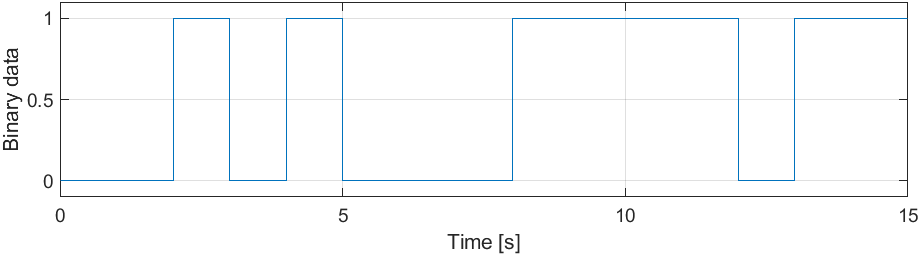
\includegraphics[width = .7\textwidth]{lab-5/imgs/initial-data.png}
\end{figure}

\FloatBarrier\noindent After running the script for the BASK technique, two signals will reasonably be displayed: the disturbed signal and the matched filter output. Noticeably, there is a threshold horizontal red line that highlights half of the carrier energy ($\frac{E_b}{2}$): if the signal exceeds the threshold a 1 symbol is detected.

\begin{figure}[h!]
    \centering
    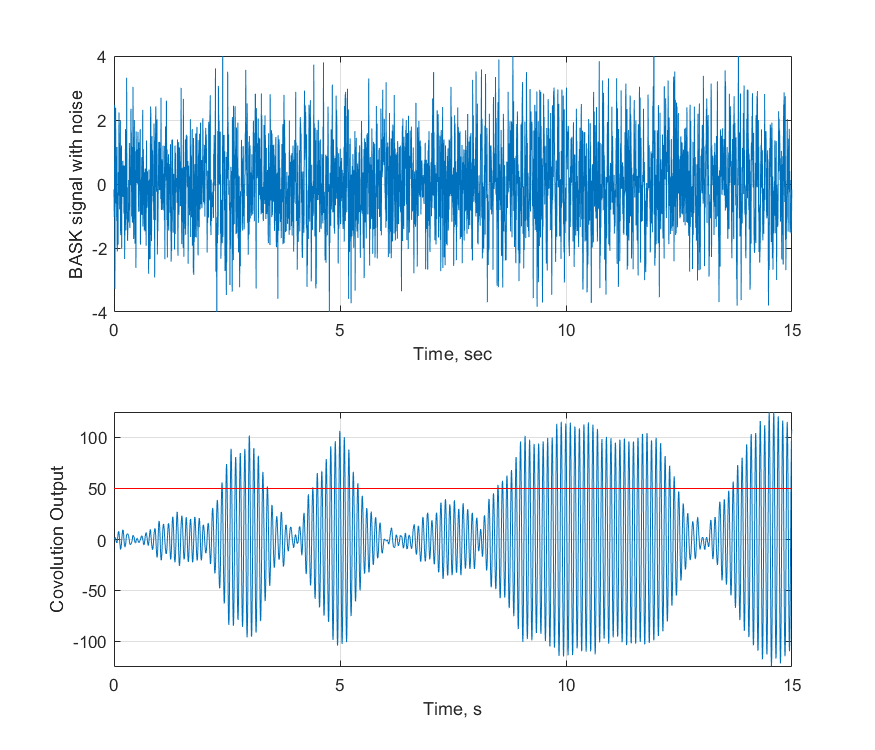
\includegraphics[width = .7\textwidth]{lab-5/imgs/BASK.png}
\end{figure}

\FloatBarrier\noindent In the BFSK modulation technique there will be two matched filters displayed, one for each carrier signal. Noticeably, when one matched filter is high, the other one is low: this difference will be crucial for symbol detection.

\begin{figure}[h!]
    \centering
    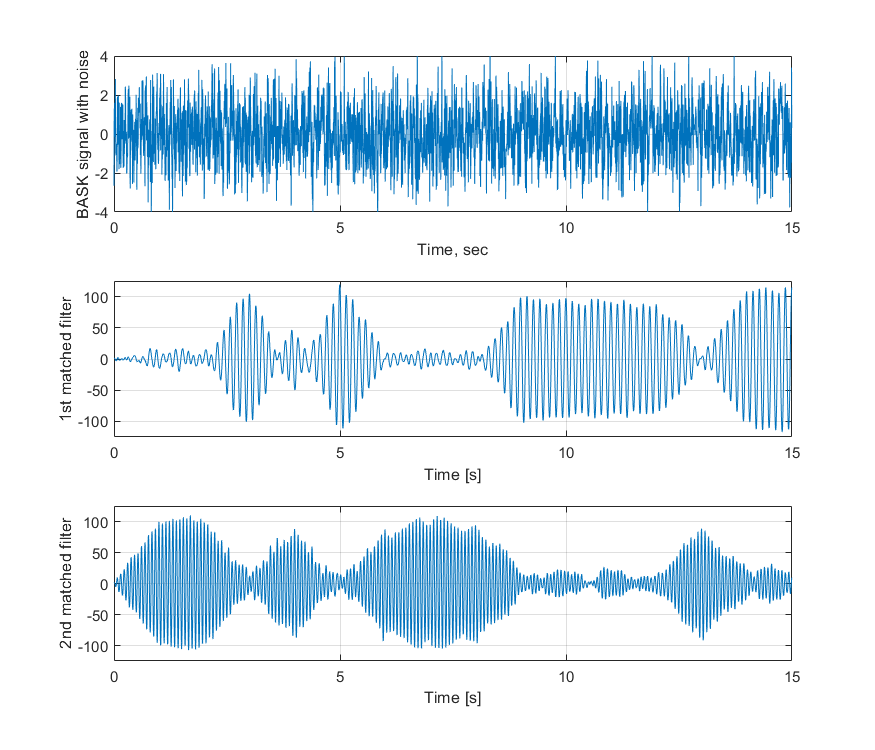
\includegraphics[width = .7\textwidth]{lab-5/imgs/BFSK.png}
\end{figure}

\FloatBarrier\noindent The third modulation technique to plot is the BPSK: in this case, as we will see, the 1 symbol is detected when the signal is lower than the zero threshold.

\begin{figure}[h!]
    \centering
    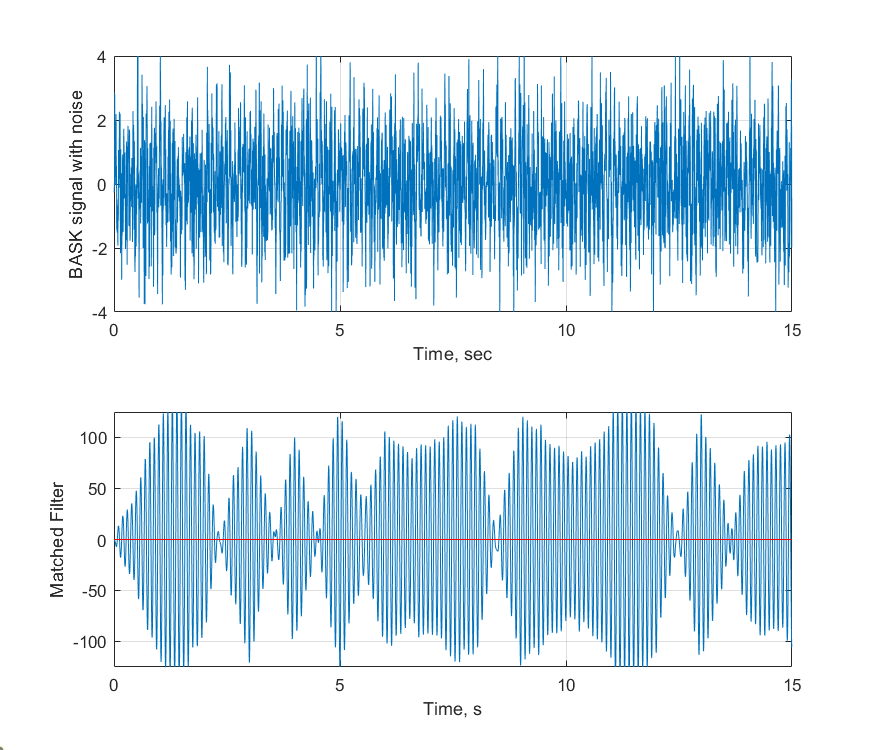
\includegraphics[width = .7\textwidth]{lab-5/imgs/BPSK.png}
\end{figure}


\subsection*{Task 3}
Task 3 asked to perform the signal detection and then compare the results with the initial data source. As we have shown previously the three modulation techniques have three different approaches to detect the symbols. Nonetheless, in all three approaches, the convolution signal is sampled using the length of the carrier $s_0$. In the BASK modulation, after computing the aforementioned steps, signal detection is achieved by comparing the matched filter output with half of the carrier energy threshold.

\begin{lstlisting}
% Perform symbols detection
L = length(s0); % length of carrier signal
sampled_signal = convolution_signal(L : L : end);
detected_symbols = sampled_signal > Eb / 2;
\end{lstlisting}

\noindent In the BFSK, after sampling both $s_1$ (for the 1 symbol) and $s_2$ (for the zero symbol) carriers signal, symbol detection is performed by comparing the first carrier $s_1$ with the second carrier $s_2$. 

\begin{lstlisting}
% Perform symbols detection
L = length(s1);
sampled_signal_1 = convolution_signal_1(L:L:end);
sampled_signal_2 = convolution_signal_2(L:L:end);
detected_symbols = sampled_signal_1 > sampled_signal_2;
\end{lstlisting}

\noindent With the BPSK modulation technique, the detection of the symbols is performed by comparing the sampled signal with the zero threshold. Specifically, if the signal is lower than zero, a 1 symbol is detected. 

\begin{lstlisting}
L = length(s0); % length of carrier signal
sampled_signal = convolution_signal(L : L: end);
detected_symbols = sampled_signal < 0;
\end{lstlisting}

\vspace{10px}\noindent Now that the symbol has been detected, it is important to analyze how many errors have occurred during the transmission. This easy operation can be achieved by the same code used in the fourth laboratory work. An element-wise check between the detected symbols and the source data shall be performed. After that, the errors can be counted by adding up the number of different symbols between the source and the detected data. At this point, it is possible to calculate the Bit Error Rate too.

\begin{lstlisting}
check = binary_sequence == detected_symbols; % check element-wise
errors = N - sum(check); % counts errors
BER = errors / N; % calculates Bit Error Rate

disp('SNR:              ' + SNR);
disp('Total symbols:    ' + N);
disp('Errors:           ' + errors);
disp('BER:              ' + BER);
\end{lstlisting}

\noindent To analyze the impact of the SNR value during the transmission, a set of 10000 symbols will be transmitted with different SNR values. The results obtained are summed up in the following table.
\begin{table*}[h!]
    \centering
    \renewcommand{\arraystretch}{1.5}
    \begin{tabular}{|c|c c c|}
        \hline
        \multirow{2}{*}{\textbf{SNR} value} &  \multicolumn{3}{c|}{\textbf{BER} value} \\
        & \textsl{BASK} & \textsl{BFSK} & \textsl{BPSK} \\\hline\hline
        20 & 0 & 0 & 0 \\
        15 & 0 & 0 & 0 \\
        10 & 0.0119 & 0.0008 & 0 \\
        7 & 0.0573 & 0.0151 & 0.001 \\
        5 & 0.1084 & 0.0349 & 0.0067 \\
        2 & 0.1837 & 0.1022 & 0.0383 \\
        0 & 0.2329 & 0.1564 & 0.0783 \\\hline
    \end{tabular}
    \renewcommand{\arraystretch}{1}
\end{table*}


\FloatBarrier\section*{Conclusions}
By analyzing the table that contains the BER values associated with the SNR values we can see a drastic increase in the error rate as the signal gets weaker, specifically in the BASK and BFSK modulations. On the other hand, the BPSK seems to be more resilient. By making a quick comparison, when the signal is 10 times stronger than the noise, using the BASK modulation the errors occurred are 119 while using the BPSK, the errors are zero. When the SNR decreases even more, lowering to 5, while with the BASK more than a thousand errors, with the BFSK the errors are 350 and with the BPSK only 67 errors occur out of 10 thousand transmitted symbols.

The results obtained and displayed in the above table are quite similar to the ones described in the fourth laboratory work. This is because, even though the optimal correlation receiver is more popular than the matched filter receiver, the math behind these two approaches is greatly similar: the correlation integral and the convolution integral are quite equivalent.

\end{document}